
% example for dissertation.sty
\documentclass[
  % Replace oneside by twoside if you are printing your thesis on both sides
  % of the paper, leave as is for single sided prints or for viewing on screen.
  oneside,
  %twoside,
  11pt, a4paper,
  footinclude=true,
  headinclude=true,
  cleardoublepage=empty
]{scrbook}

\usepackage{dissertation}

% ----------------------------------------------------------------

% Title
\titleA{}
\titleB{Im2Model} % (if any)
\subtitleA{Efficient computation to refine atomic models}
\subtitleB{for TEM image simulation and matching} % (if any)

% Author
\author{Filipe Costa Oliveira}

% Supervisor(s)
\supervisor{Alberto Jos\'{e} Proen\c{c}a}
\cosupervisor{Daniel Grando Stroppa}

% University (uncomment if you need to change default values)
% \def\school{Escola de Engenharia}
% \def\department{Departamento de Inform\'{a}tica}
% \def\university{Universidade do Minho}
% \def\masterdegree{Computer Science}

% Date
\date{\myear} % change to text if date is not today

% Keywords
%\keywords{master thesis}

% Glossaries & Acronyms
%\makeglossaries  %  either use this ...
%\makeindex	   % ... or this

% Define Acronyms
%%!TEX root = ../dissertation.tex

\newacronym{mei}{MEI}{Mestrado em Engenharia Inform\'{a}tica}
\newacronym{um}{UM}{Universidade do Minho}
%\glsaddall[types={\acronymtype}]


\ummetadata % add metadata to the document (author, publisher, ...)

\begin{document}
	% Cover page ---------------------------------------
	\umfrontcover	
	\umtitlepage
	
	% Add acknowledgements ----------------------------
	\chapter*{Acknowledgements}
%	Write acknowledgements here


	% Add abstracts (en,pt) ---------------------------
	\chapter*{Abstract}
	
	
	
	TEM (Transmission Electron Microscopy) is a well-established characterisation tool with wide use on
the analysis of nanostructured materials. Even though modern TEM equipment is able to reach atomic
resolution regularly, the suitable quantitative interpretation of experimental images is currently limited
due to the required extensive and complex analyses.\par 

A self-contained software solution to interpret TEM images of nano-structured materials is not currently available yet: these are often analysed in a qualitative way.


%There is currently no efficient implementation of nanostructured sample description based on a single TEM image, and TEM results are often analysed in a qualitative way. 

Only few examples of quantitative analysis of TEM images with atomic resolution are
currently present in the literature%referencia%
, reflecting the complexity and the time-consuming aspect of the
outlined analysis chain.\par 


This dissertation aims to implement a software system, named Im2Model, addressing this gap in nano-materials
characterisation. Im2Model will combine transmission electron microscopy, image correlation and matching procedures, enabling the determination of a three-dimensional atomic structure based strictly on a single high-resolution experimental image.\par 
The software architecture approach will contain well-defined boundaries, clear responsibilities, and controlled dependencies.
Performance engineering will be present in each step of the traditional software development process, 
aiming for 
both execution time-efficiency and resource usage efficiency, of the final software product.



	
	
	\cleardoublepage
	\chapter*{Resumo}
	
	
	A  Microscopia Eletr\'{o}nica de Transmiss\~{a}o (TEM) \'{e} uma ferramenta de caracteriza\c{c}\~{a}o bem estabelecida e com ampla utiliza\c{c}\~{a}o na an\'{a}lise de materiais nanoestruturados. Embora os equipamentos  TEM sejam capazes de atingir resolu\c{c}\~{a}o at\'{o}mica, a interpreta\c{c}\~{a}o adequada das imagens experimentais est\`{a} actualmente limitada devido \`{a}s extensas e complexas an\'{a}lises manuais necess\'{a}rias.\par 
	N\~{a}o existe actualmente uma ferramenta de software para interpretar imagens TEM de materiais nanoestruturados.\par 
	Existem at\'{e} ao momento poucos exemplos de an\'{a}lise quantitativa de imagens TEM com resolu\c{c}\~{a}o at\'{o}mica, reflectindo a complexidade e o extenso tempo necess\'{a}rio para a sua an\'{a}lise.\par 
	Pretendemos implementar uma ferramenta de software, de nome Im2Model, que preencha esta lacuna na caracteriza\c{c}\~{a}o de nanomateriais. O Im2Model combinar\'{a} a microscopia de transmiss\~{a}o eletr\'{o}nica  e algoritmos de correla\c{c}\~{a}o de imagem, permitindo a determina\c{c}\~{a}o de uma estrutura at\'{o}mica tridimensional baseada estritamente em uma \'{u}nica imagem experimental de alta resolu\c{c}\~{a}o. 
	\par 
	
	
	Em cada etapa do processo de desenvolvimento de software estar\'{a} presente uma vis\~{a}o de  engenharia paralalela e de alta performance, almejando a redu\c{c}\~{a}o  do tempo de execu\c{c}\~{a}o da aplica\c{c}\~{a}o assim como uma utiliza\c{c}\~{a}o eficente dos recursos de computa\c{c}\~{a}o.
	
	% Summary Lists ------------------------------------
	\tableofcontents
	\listoffigures
%	\listoftables
	%\lstlistoflistings
	%\listofabbreviations
	
	
	\pagenumbering{arabic}
	
	% CHAPTER - Introduction -------------------------
	\chapter{Introduction}
	\section{Context}
	
	
%	Understanding the correlation between physical properties and nanostructured materials is a long-standing goal in science. 
	Nanostructured materials (including nanoparticles) may exhibit new physical properties or new behaviours. Although some of these properties are already known, there may be many more unique physical properties not known to us yet, showing an extremely broad range of potential applications in several areas of research.\par 
	
		%change order and reduce 
	Research on new physical properties and applications of nanostructured materials is possible only when nanostructured materials are made available with desired morphology, size, and atomic composition. 
	
	

	
%	In crystalline materials, where atoms are situated in a repeating or periodic array over large atomic distances,
%	it characterisation has been largely based on the surface analysis techniques and conventional characterisation methods developed for bulk materials.
	\par 
    Transmission electron microscopy (TEM) has been commonly used in characterisation
of nano-structured materials, elucidating the nanometer scale structures. 
However, it has a serious drawback due to the fact that electron scattering information in a TEM image originates from a three dimensional
sample but is projected onto an two-dimensional detector.\par 
The structure information along the electron beam direction is superimposed
at the image plane, therefore the information along the thickness direction of the sample is only an accumulated one leading to possibly resulting in tricky interpretations, pose a problem in reconstructing 3D images based on single high-resolution TEM images.\par 

%This holds for both instrumental modes , the coherent imaging mode (TEM) and the (STEM).\par

 On the scanning mode of transmission electron microscopy (STEM) methods have been developed, like the High-Angle Annular Dark Field (HAADF), that allow the 3D reconstruction of the nano-structured material based on a single image. For the coherent imaging mode (TEM) the satisfactory solution for 3D reconstruction still relies on several high-resolutions images, taken in different orientations, of the same sample.\par 
 Figure \ref{fig:tem_2_atom_Ce02} illustrates the desired sample input and output of application to be developed.

\begin{figure}[h!]
	\begin{center}
	
	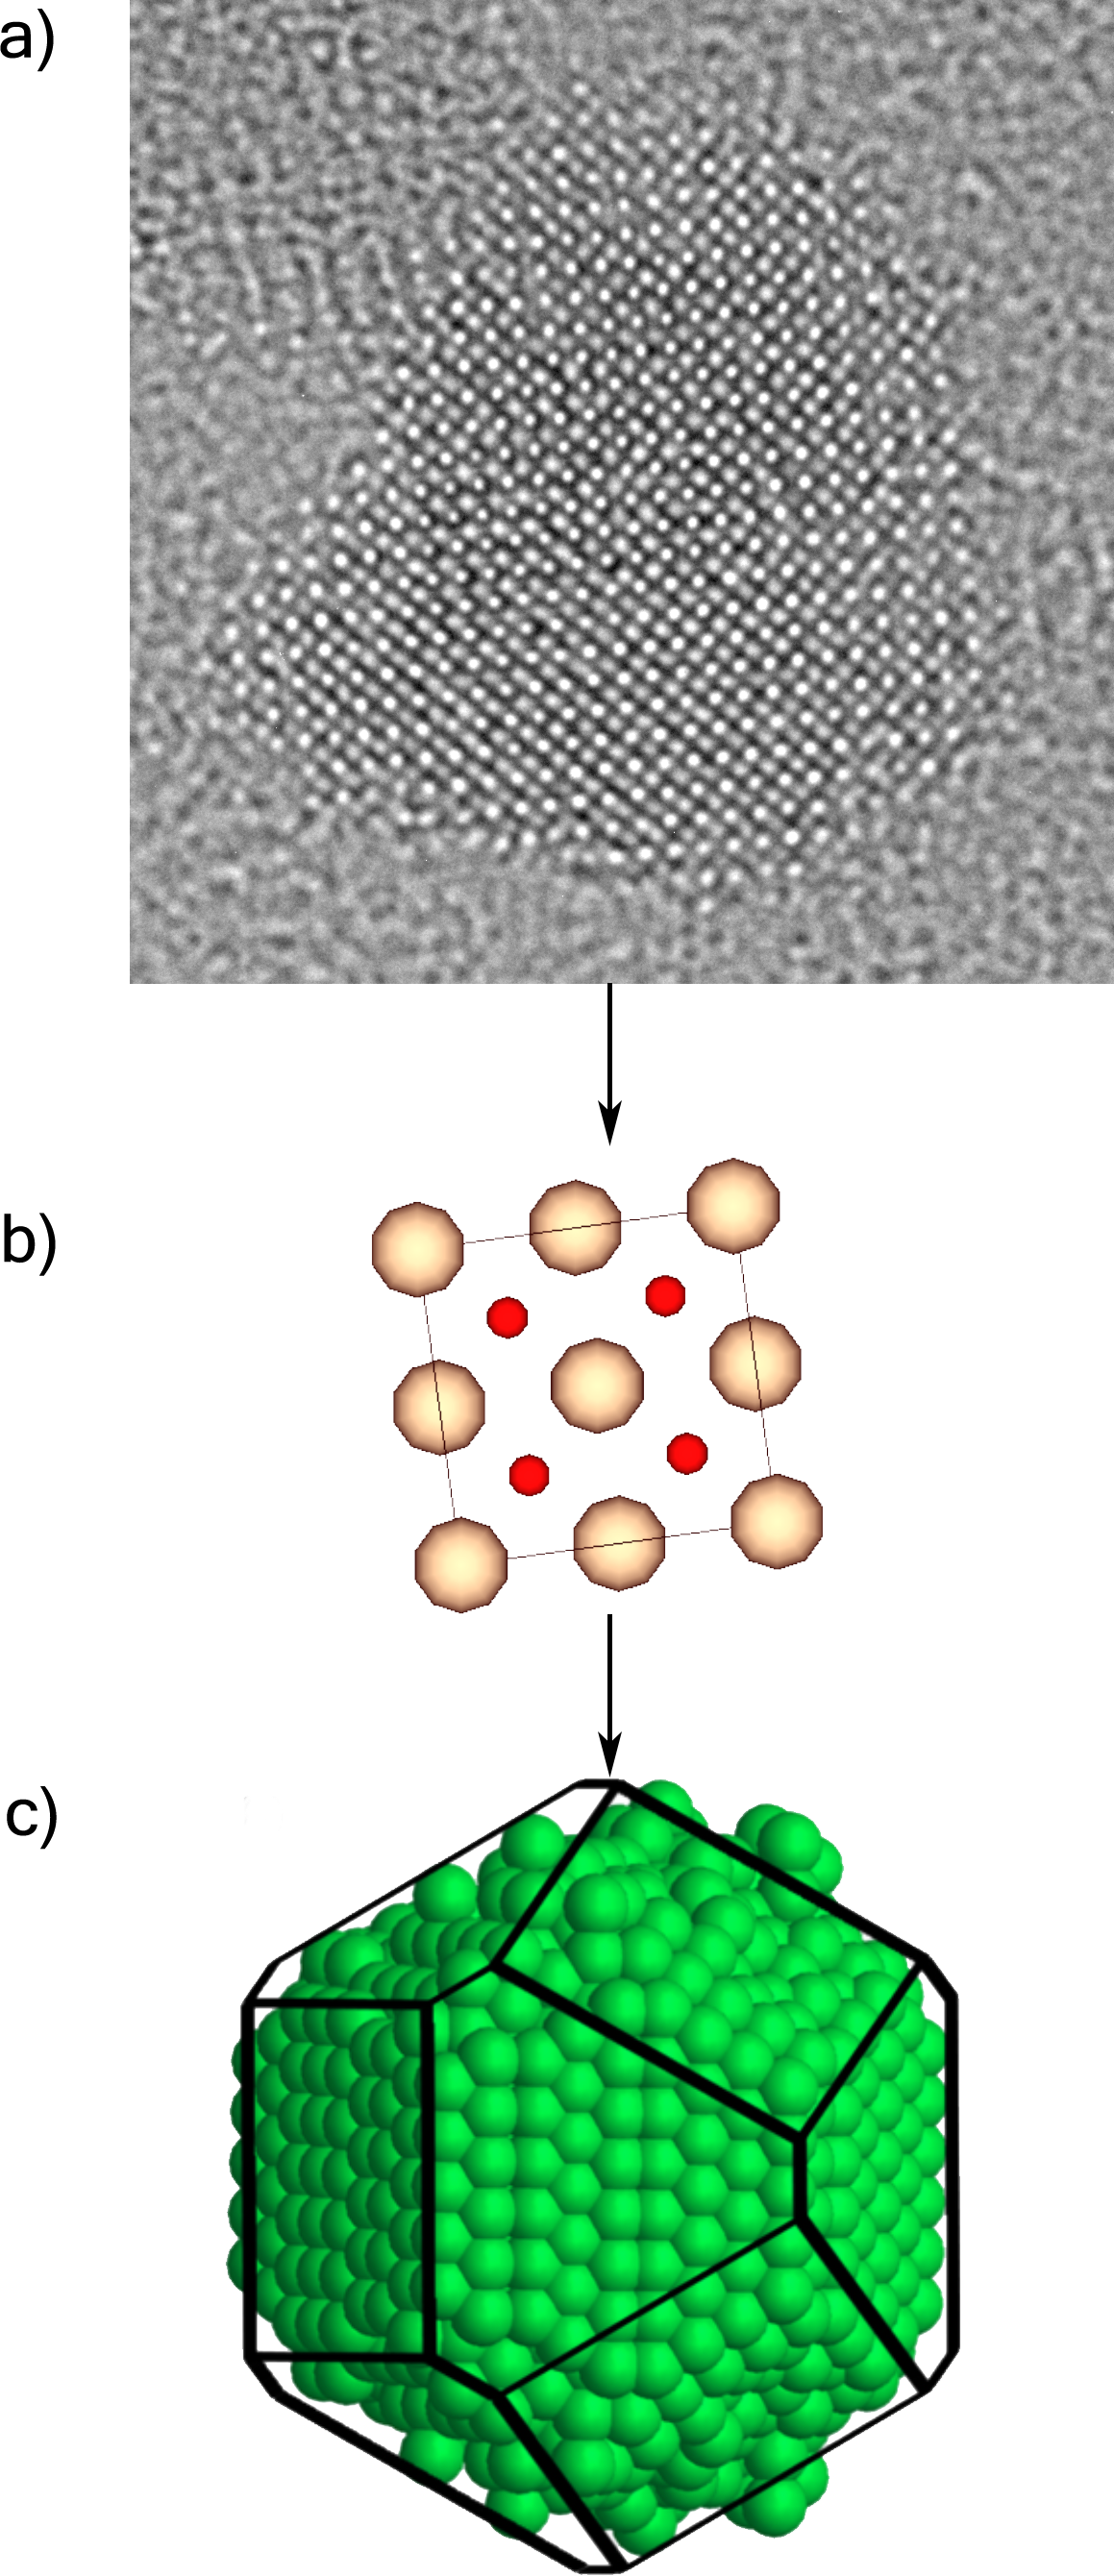
\includegraphics[width=0.3\textwidth]{img/Im2Model_goal.png}
			\caption[Desired sample input and output of Im2Model]{Desired sample input and output of Im2Model.\splitter
			\newline
			a) 2D-TEM image of a CeO2 (cerium oxide) crystal.\newline
			b) Given crystallographic indexing and orientation information.\newline
			c) Example 3D-TEM reconstruction of a CeO2 (cerium oxide) crystal.}
	\label{fig:tem_2_atom_Ce02}
		\end{center}
	\end{figure}
	
 






	\section{Motivation}
	
	Even though modern TEM equipment is able to reach atomic
resolution regularly, the suitable quantitative interpretation of experimental images is currently limited
due to the required extensive and complex analyses.\par 

	There is currently no efficient implementation of the preceding method and TEM results are often analysed in a
qualitative way. 
Only few examples of quantitative analysis of TEM images with atomic resolution are
currently present in the literature %%% inserir referencia,
reflecting the complexity and the time-consuming aspect of the
outlined analysis chain.\par 
Moreover, more accurate representations and higher resolution models are directly associated with the usage of simulation for the physical processes. HPC is now an integrant component of the nanostructure materials studies, with simulations presenting ever increasing scales.\par



	\section{Contribution}
	
	To address the presented problem, the introduction of an automated software tool capable of automating the structural information acquisition from coherent transmission electron microscopy imaging mode (TEM) of nanostructured materials, producing a three dimensional atomic model of the observed sample, will greatly reduce the time needed for the analysis of experimental images.\par 
	
	The possibility of creating an atomic model from a single high-resolution TEM image would increase the information presented to electron microscopy users and would support the automation of tasks and information retrieval(currently retrieved manually).\par 
	
	The software tool to be developed, named Im2Model, is therefore presented as a bridge between data visualisation of nano-structured materials crystallographic information and quantitative interpretation in a real-time basis of experimental attained high-resolution TEM images.\par 
	
	
	
		\section{Dissertation Structure}
		
This dissertation has 7 chapters, each with their summary presented bellow.
The first 3 chapters go through the fundamental ideas that apply to both scientific software and high performance software, whether running on a single machine or distributed across a cluster of machines.


\begin{itemize}
    \item \textbf{Introduction}: Presenting the motivation for this dissertation, and illustrating the desired sample input and output of Im2Model.
    

    
     \item \textbf{Atomic Models for TEM Image Simulation and Matching}:
    Presenting the state-of-the-art regarding the  crystallographic indexing of nano-structured materials,  methodologies for TEM image simulation, and image correlation algorithms, presenting us to the internals of scientific simulation.
        
    \item \textbf{Computational Efficiency}:  Presenting the state-of-the-art art in terms of hardware and
software performance metrics and modelling.

    It examines what we actually mean by words like efficiency and scalability, and how we can try to achieve these goals.
    
    \end{itemize}
    
    Later, the following 4 chapters will turn to the particular issues of the simulation of the described physical process in distributed data systems.
\begin{itemize}

    \item \textbf{The Product}:
    Describing in detail the current solution legacy systems dependencies, and dividing different models and their components by their specific Ubiquitous Language and forming multiple Bounded Contexts.\\
    

    
    \item \textbf{Efficient implementations of Im2model workflow}:
    
    
    The previously described architecture, had functionality built on the same machine. These functional groups are tightly coupled, symbiotic systems. They depend on local, shared resources like disk, network interface, or inter-process communications. \par

    This chapter focus on modelling and implementing the system to achieve the level of reliability, agility, and scale expected, built out of many different components running in different processes and communicating over distinct means spread across multiple machines, 
    with elastic \/ on-demand resource allocation. We will also be focusing attention on the resources that are exchanged between Bounded Contexts.\par
    Considering we are modelling software to runs on several machines, connected by several distinct networks, faults and failures will be also taken in account in the design and implementation stages. We are no longer operating in an ideal system model, but in nondeterministic one with the possibility of partial failures. Therefore, we will discuss a wide range of problems that can occur in the modelled distributed system.    \par

    
        \item \textbf{The test boundary}:  
        
        This chapter dives into the different types of tests we have run to effectively and efficiently test the system functionalities when they spanned into a distributed system, while also breaking down the problems associated with testing finer-grained systems. It presents an overview of the  results obtained by
the preliminary experimental work developed.

            \item \textbf{Conclusion}: Presenting an overview of  Im2Model major challenges until the current developing stage and future steps.


\end{itemize}





	% CHAPTER - State of the Art ---------------------
	\chapter{Atomic models for TEM image simulation and matching}

	\section{Related work}
	
	The conventional electron tomography method to determine the three-dimensional structure of the nano-structured material relies on a number of images taken along different viewing angles \citep{batenburg20093d}. 
The acquisition of several high resolution images may add inaccuracy to the consistent reconstruction of the model, since the physical properties of the nano-structured material 
may be modified due to the high-energy electron beam required by TEM tomography. These small modifications on the acquired images may lead to different nanostructure reconstructions.\par 

The 3D shape of several nanostructured materials has been reconstructed  with a significant reduction of the required slice images, by using a discrete tomography technique in
STEM \citep{jinschek20083}.
\par 
%On account of the STEM process generating the high-resolution pixel by pixel, the produced intensity of each pixel in High-Angle Annular Dark-Field  imaging  technique (HAADF) proves ideal for atomic reconstruction\citep{jia2014determination}, as it generates strong contrast that has a non-linear relation to the thickness of the of the atomic structure observed. 

The scanning process pixel by pixel in STEM generates high-resolution images. The captured intensity from each pixel in a High-Angle Annular Dark-Field imaging technique (HAADF) proves ideal for atomic reconstruction\citep{jia2014determination}. It generates strong contrast that has a non-linear relation to the thickness of the observed atomic structure.\par 
For TEM images this process can not be used, due to wave interferences registered on the captured image. To overcome this problem the current applied method uses an atomic structure model 
and a simulation of optical parameters,
 varied stepwise in such a way that the image calculated
on this basis provides a best fit to the experimental image. 
 With the comparison of the simulated images with the experimental image is determined if the model has a good approximation or not from the sample used. 
 This method can be applied for both instrumental modes of TEM, being the most reliable process for atomic structure reconstruction.
	
	\subsection{Nanostructured materials crystallographic indexing from high resolution (S)TEM images}
	
	A precedent step of high resolution TEM image simulation is the characterization of nanocrystalline materials at higher resolutions as obtainable in a transmission electronmicroscope (TEM). Nanostructured materials crystallographic indexing refers to labeling the diffraction rings and spot with appropriate Miller indices (hkl).\par 
	 Crystallographic indexing of  using high resolution (S)TEM images
	 can be carried out manually by the users by application of the reciprocal lattice and kinematical theory of electron diffraction, resulting in a reduced TEM characterization yield and significant user bias.\par 
	 There is an alternative (S)TEM technique that works on the basis of a new software tool to aid the crystallographic indexing of nanostructured materials using high resolution (S)TEM images. Im2Cr \citep{asilva2016} implementation aims for a minimal user interaction, supporting the detection of zone-axis oriented particles, and including an efficient peak detection process applied to the images Fourier Transform (FT). With basis on the FT peaks distances and relative angles, crystallographic indexation is carried out autonomously via comparison with a list of candidate structures named by the user, and a ranking of the best matching combinations of crystallographic structures and viewing zone axes are generated. This technique provides efficient and reliable data analysis reducing the complexity and time needed to to produce a crystallographic analysis. Figure \ref{fig:im2cr_worflow} illustrates the Im2Cr workflow. 

\begin{figure}[!ht]
	\begin{center}
	
	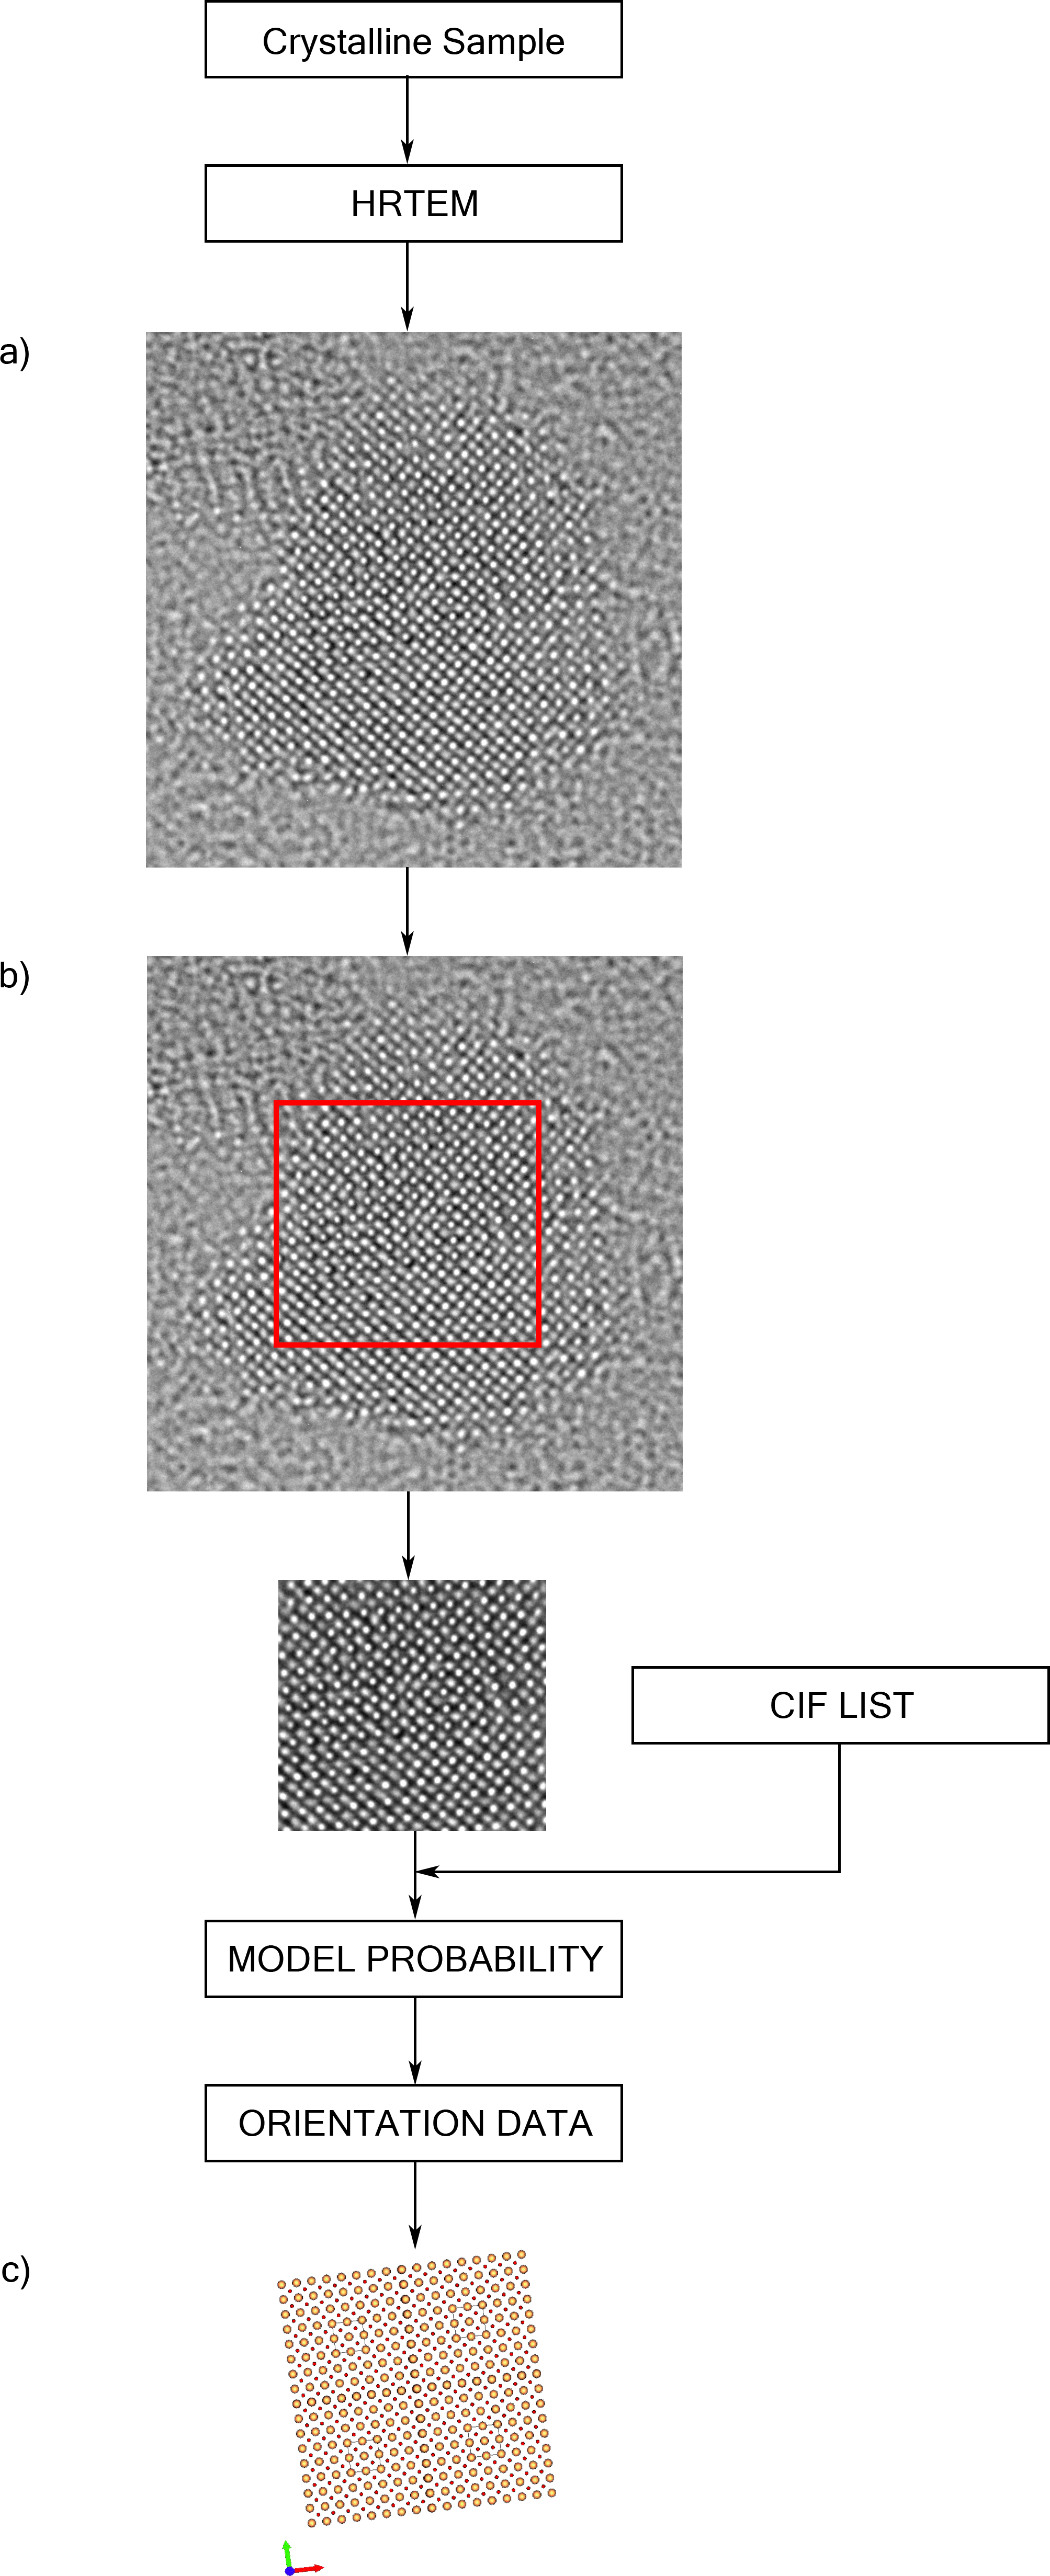
\includegraphics[width=0.5\textwidth]{img/Im2Cr_workflow.png}
			\caption[Im2Cr workflow]{Im2Cr workflow.\newline 
			a) 2D-TEM image of a CeO2 (cerium oxide) crystal.\newline
			b) Selected ROI from the 2D-TEM image.\newline
			c) Generated crystallographic structures and viewing zone axes.}
	\label{fig:im2cr_worflow}
		\end{center}
	\end{figure}
	
	\clearpage

	
		\subsection{TEM image simulation}
		
		Transmission electron microscopy image simulation is essential in TEM characterisation of nanostructured materials.
		Here, the nanostructure is sectioned into thin layers along the direction of the electron beam. Each layers is prepensed to represent a narrow height interval of the nanostructure, which allows the weak phase object approximation for the calculations at each layer. The multislice algorithm becomes exact only in the limit of very thin layers.\par 
		
		The scattered wave is then propagated in vacuum to the next layer and the process is repeated until the desired sample thickness is reached.
		
		Is fundamental for the simulation software to employ a multislice simulation method capable of including the effects of geometrical aberrations (image properties), and 
  wavefront aberrations (transfer function properties).\par 
		
		Due to the crystalline materials long range order property, 
		super cells are utilised to  simplify the TEM multislice simulation input with respect to the atoms information.\par 
		
		There exist a number of free as well as commercially available software  based on the multislice algorithm for conventional TEM image simulations:
		\begin{enumerate}
				    \item Dr. Probe \citep{drprobe}
		    \item QSTEM \citep{koch2002determination}
		    \item JEMS \citep{stadelmann2014java}
		    \item MacTempas \citep{kilaas2014mactempasx}
		    \item STEM\_CELL \citep{stemcell}
		\end{enumerate}
		
		The multislice simulation will be carried out using Dr. Probe \citep{drprobe} %%pf verificar referencia
		command-line software tools, composed of three tools, each related to one of the three Dr. Probe simulation steps.  This separation gives birth to future work-flow optimisations when doing parameter variations, as not all steps need to be repeated depending on the level where the parameter variation takes place.

		
	\subsection{Image correlation}
	
	Algorithms for aligning images are among the oldest and most widely used in computer vision.	One of the most commonly used algorithm is to shift or warp the images relative to each other and to look at how much the pixels agree, directly minimising pixel-to-pixel dissimilarities, normally refered as  the patch-based translational alignment \citep{lucas1981iterative}. 
	A variety of such parametric motion models are possible, from simple 2D transforms, to most complex 3D perspective transformations.\par 
	To use the precedent method, a suitable error metric must first be chosen to compare the images, which normally is achieved recurring to one of the following image similarity metrics\citep{brown1992survey}:
	
	\begin{itemize}
	    \item \textbf{Squared difference} -- Match the squared difference of the patch and the input image.
			Perfect match will be 0, and bad matches will be large.
	     \item \textbf{Cross Correlation} -- Multiplicatively match the patch against the input image.
			Perfect match will be large, and bad matches will be small or 0.
			
	     \item \textbf{Correlation Coefficient} -- Match the patch relative to its mean, against the input image relative to its mean.
			Perfect match will be 1, and a perfect mismatch will be -1. 0 represents random alignments.
	\end{itemize}
				

We should obtain more accurate matches, at the cost of more computation effort, as we move from simple measurement methods like the squared difference, to more sophisticated ones like correlation coefficient.\par
The normalised methods of the precedent error metrics are extremely useful since they help reducing the effects of lightning differences between the images being correlated.\par 


Computer vision operations will be carried out by recurring to the free Open Source Computer Vision Library (OpenCV) that optionally can be highly optimised by loading the commercial Intel Integrated Performance Primitives (IPP)\citep{ˆome2004programming}, or developing GPU-accelerated image processing that will be integrated with native OpenCV C++11 methods.




\section{The Im2Model Work-flow}

To achieve the Im2Model goal, a preliminary crystallographic analysis of TEM images will be carried using the Im2Cr software, recently 
developed at UMinho \citep{asilva2016}. Im2Cr provides the most likely crystalline structure and its orientation from a single region of interest in an experimental image. \par 
A validation step will be then carried out through an image simulation of a small segment and its
comparison with the experimental image. This procedure is often referred as thickness-defocus maps in
TEM simulation. This step will be carried out using Dr. Probe \citep{drprobe} 
software, and (i) will confirm the
crystallographic indexing by Im2Cr \citep{asilva2016}, (ii) validate the experimental setup parameters informed by the
user, and (iii) estimate the local sample thickness.\par 
A super cell model representing the whole structure will be built based on the crystallographic structure
retrieved by Im2Cr \citep{asilva2016} and the estimated dimensions of a certain region of interest. Iterative steps of image
simulation, images comparison and model refinement will be carried out until a convergence threshold.\par 
During these steps, the atomic model and the TEM experimental parameters will be refined, leading to a
complete description of the sample structure.\par 



Figure \ref{fig:tem_modeling_workflow} illustrates the high-resolution TEM modelling workflow, including the preliminary phases required as Im2Model input parameters, provided by Im2Cr \citep{asilva2016} and by the experimental results. \par 


\begin{figure}[!ht]
	\begin{center}
	
	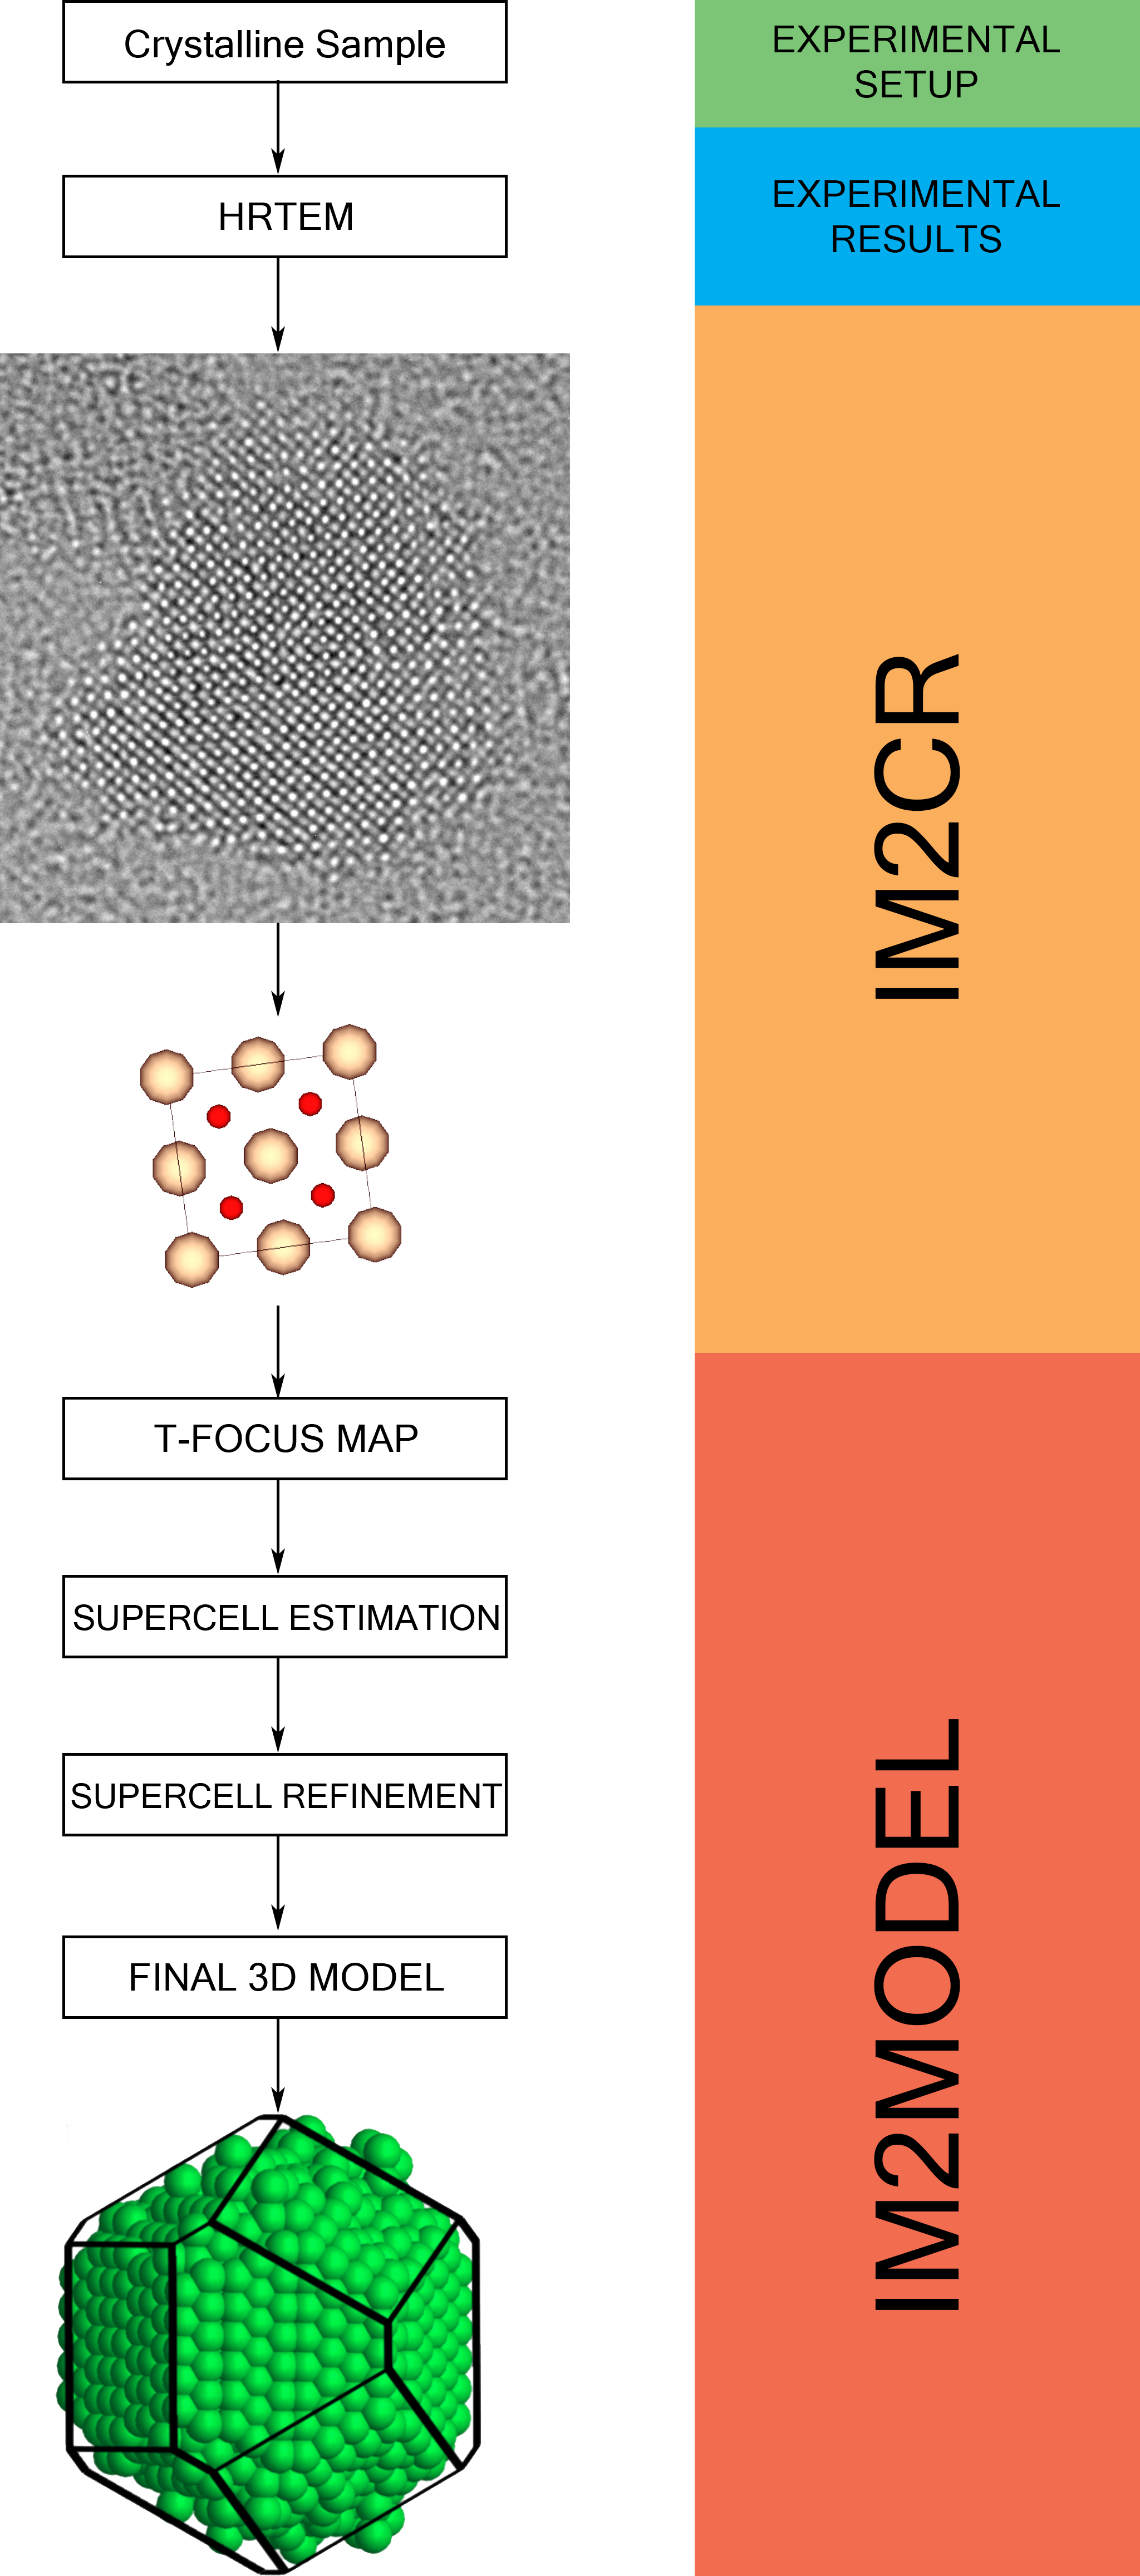
\includegraphics[width=0.5\textwidth]{img/workflow.png}
			\caption{High resolution TEM modeling workflow}
	\label{fig:tem_modeling_workflow}
		\end{center}
	\end{figure}
	
	\FloatBarrier
	
	\label{chapter:workflow}
	
	
The integration and refinement of the resulting application code and associated data structures will
follow efficiency methods to lead to faster execution times and optimum resource usage, taking
advantage of code vectorization, data locality (both NUMA and cache levels), code parallelism (both
thread-level and process-level) and computing paradigms (using computing accelerators, such as Intel
MIC devices and NVidia GPUs). If such levels of efficiency are reached, it could open new horizons regarding the use of TEM technology.



\label{chapter:im2model_workflow}


	% CHAPTER - Problem and Challenges ---------------
	\chapter{Computational efficiency of Im2Model}

\section{Performance: goals and its modelling} %% Target Optimization Metrics


A performance goal provides direction for our performance analysis work and will 
help the optimisation pipeline. Our main objective is to provide a time-efficient and
unbiased work-flow for the quantitative interpretation of high-resolution TEM images, by the use of
efficient computation methods, enhancing the productivity on materials characterisation at the atomic
scale. Considering that the work-flow presents such a demanding and wide-ranging requirements, a single approach can no longer meet all of its computing, data processing and storage needs. 
Instead, the work is broken down into smaller tasks that can be performed efficiently, and those different tools are stitched together using an distributed system design approach.\\

The composite distributed system must provide certain guarantees:

\begin{enumerate}
				    \item Reliabitity
		    \item Scalability
		    \item Maitainability
		\end{enumerate}


The resource utilisation efficiency for a given application workload
can be considered as the secondary objective.\par 





\section{Describing Performance} %% Target Optimization Metrics

This chapter will refer to some commonly used techniques by which application performance
can be improved: selecting an I/O size, caching, buffering, concurrency
and parallelism, non-blocking I/O, and processor binding. Some of them are strictly related to the target platforms and to the target operating systems. \par 
Performance issues can arise from
anywhere, including software, hardware, and any component along the data path. Its is important to include when available and applicable, network, operating system, file system, memory, and CPU performance analysis which can also identify application level
issues.

\section{Target Platforms}

Concerning the computational efficiency evaluation of Im2Model the target platform should extend the hardware performance limits to the maximum. Therefore clustering environments are ideal for high performance computing development.\par 
The SeARCH6 cluster at the University of Minho (Services and Advanced Research Computing with HTC/HPC clusters) is a computing infrastructure containing 800 cores distributed over 54 nodes with dual Intel Xeon processor. Each node contains two multi-core CPU devices, either Ivy Bridge processors (E5-2650v2, E5-2670v2, E5-2695v29) or Nehalem processors (E5520, X5650, E5649),
and eventually one or more computing accelerator, for example, a GPU (Graphics Processing Unit) or a many-core CPU device, such as the Intel Many Integrated Cores (MIC) device. 

Regarding the coprocessors and computing accelerators distribution SeARCH6 has 21 accelerators distributed over 12 nodes: 9 Intel Xeon Phi (8×7120 1×5110 and) and 12 NVIDIA Tesla (5x K20m Kepler, Fermi M2090 1x, 2x and 4x Fermi M2070 Fermi C2050).\par 

The access time for main memory is non-uniform (NUMA) -- therefore
varies based on its location relative to the CPU memory architecture for each two-processor computing node. The main memory amount ranges from 8 to 64GB, with 28 nodes possessing the largest configuration. 
The speed of the memory bus, for any architecture, is often dictated by the memory interface standard supported by the processor and system board. Therefore it should be evaluated based on the CPU units description.\par 

Disk I/O can cause significant application latency and is therefore an important target of systems performance analysis. 
Flash-memory-based solid-state disks with 240GB will be the main storage system for each computing node. A distributed Network-Attached storage system of 98TB is integrate in the cluster environment, consisting of Dot Hill SAN with 40TB of raw capacity, connected by 16Gbit/s Fibre Channel links to 4 dual-Xeon nodes, each with 12TB of raw capacity. These nodes also facilitate access to the entire storage space via NFS and GlusterFS.\par 

Two network interfaces are available across the cluster, one with low latency 10 Gbit/s Mirynet, and another 1 Gbit/s Ethernet.\par 

In order to obtain the best performance possible the described clustering platform will be used in the evaluation of performance in the  development and testing stages. In the production stage the application is to be run on desktops or laptops, normally present in TEM laboratories.\par 
Despite the described clustering environment possessing features above the currently used laptops, the evolution of the computer systems will soon match or overcome these characteristics.

\section{Target Operating Systems}
An understanding of the operating system and its kernel is essential for systems
performance analysis. The SeARCH6 cluster is based on the Rocks 6.1 cluster management distribution, a Linux distribution intended for high-performance computing environments.\par 

Other Unix based distributions will also be validated for later development stages, as well as a Microsoft Windows version.

\section{Transformation for Performance}


There are a number of possible user-level optimizations that have been found effective for ultimate performance. It is unlikely that peak performance will be achieved without considering some of these optimizations:

\subsection{Data Parallelism}

\subsubsection{Vectorization}

Vector instructions are a special set of intructions based on the Single Instruction Multiple Data (SIMD) model, where a single instruction is simultaneously applied on multiple data.\par 

In previous generations of processors, vectorization of operations was of lesser importance, mainly because of the shorter vector units. With the arise of 256-bit and 512-bit long vectors utilization is increasingly necessary to achieve high performance.\par 

This has drawn the auto-vectorization capabilities of modern compilers into focus, however such compilers at best could only vectorize a few classes of applications with regular memory access and computation patterns, such as structured grids or multimedia.\par 

Gaining good performance from vector units is not only important for CPUs but also for emerging co-processors. 
Very explicit programming techniques specific to the hardware are required to gain maximum performance.

\subsection{Data Alignment}

    Vectorization works best on unit-stride vectors, the data being consumed is contiguous in memory. 
    Data structure transformations can increase the amount of data accessed with unit-strides and should therefore be considered.
    
\subsection{Memory access and loop transformations}

\subsubsection{Cache Optimisation}

The most effective use of caches comes by paying attention to maximising the locality of references, blocking to fit in L2 cache dimensions present on the SeARCH6 processors, and ensuring that prefetching is utilised (by hardware, by compiler, by library or by explicit program controls).


\subsection{Processor Binding}
For NUMA environments like SeARCH6 compute nodes, it can be advantageous for a process or thread to remain
running on a single CPU and to run on the same CPU as it did previously after
performing I/O. This can improve the memory locality of the application, reducing
the cycles for memory I/O and improving overall application performance.

\section{Parallelization approaches}

Time-sharing systems provide 
the ability to load and begin executing multiple runnable programs, vulgarly described as program concurrency. While
their runtimes may overlap, they do not necessarily execute on-CPU at the same
instant. Each of these programs may be an application process.\par 

Apart from executing different applications concurrently, different functions or code sections
within an application can also be made concurrent. This can be achieved using
multiple processes (multiprocess) or multiple threads (multithreaded), each performing
its own task.\par 

Frameworks for parallelising both on shared and distributed memory paradigms are presented next.


\subsection{Shared Memory Parallelism}

\subsubsection{Posix Threads (PThreads)}


Pthreads programming model is part of the C programming language and composed of programming types and procedure calls, that get called and included by a pthread.h header thread library. \par 
To fully exploit the computational potential presented by Pthreads, a program has to be structured into distinct autonomous processes which then get implemented and run in parallel. \par
Posix Threads are composed of  sub-routines, mainly classified as thread management, mutexes,
condition variable, and synchronization sub-routines.

\subsubsection{OpenMP 4.5}

OpenMP is a portable, scalable model that gives parallel programmers a simple and flexible interface for
developing portable parallel applications. OpenMP is primarily designed for shared memory multiprocessors, taking a directive-based approach for supporting paralellism, allowing the same code base to be used for single-processor and multiprocessor computing platforms, and promoting an incremental approach to parallelism.\par 
The latest versions of OpenMP standards have introduced a number of new directives designed to support heterogeneous computational offloading in order to target many-core devices, while also enabling multiple levels of parallelism. The developer can now describe a group of thread teams, and then distribute the iterations of a loop to the master threads in each team. Depending on the target, this could place threads on the cores of a CPU, or block them onto the streaming multiprocessors of a GPU or coprocessor.

\subsubsection{Intel Thread Building Blocks (TBB)}

Intel Threading Building Blocks (TBB) is a C++ template library allowing the programmer to decompose computation into tasks that can be created dynamically at run time.

The programmer does not need to be concerned with dividing the computation evenly among a fixed number of threads. Instead, TBB promotes the practice of breaking down the computation into tasks of appropriate granularity. \par 
The tasks are submitted to a task pool and the Task Scheduler dispatches the tasks to the hardware units in an efficient way. 
Moreover, TBB implements a task stealing mechanism that takes into account task data locality and
system's workload, making it suitable for applications having tasks with unpredictable execution time and thus very difficult to balance manually. Both functional and data parallelism are supported by TBB.



\subsubsection{Intel Cilk Plus}
Intel Cilk Plus extends C and C++ to enable writing composable deterministic parallel software that can exploit both the thread and vector parallelism commonly available in modern hardware.
Cilk Plus breaks the algorithm into independent computations (tasks)
and handle allocation of tasks to threads during run-time to ensure efficient execution. The explicit vector language makes it easier to exploit SIMD instructions efficiently.\par 
It maintains a stack with
the remaining workflow, employing a work stealing heuristic similar to the prior described Intel TBB.





\subsection{Distributed Memory Parallelism}

\subsubsection{Compute Unified Device Architecture (CUDA)}


Based on the CUDA architecture, NVIDIA GPUs
 with the new Tesla unified graphics and computing architecture run CUDA C/C++ programs and are widely available in laptops, PCs, workstations, and servers.\par 
 
CUDA provides three key abstractions --
a hierarchy of thread groups, shared memories, and barrier synchronization, that provide a clear parallel structure to conventional C code for one thread of the hierarchy.\par 

Multiple levels of threads, memory, and synchronization provide data parallelism nested with thread and task parallelism.\par 
 
 
\subsubsection{Message Passing Interface (MPI)}

The Message Passing Interface (MPI) provides a simple API for parallel programming in
distributed memory environments, with the main goals being high performance, scalability, and portability. 
Both point-to-point and collective communication are supported.\par 

Most MPI implementations consist of a specific set of routines directly callable from C, C++, Fortran. The data must be explicitly split and passed among the processes
by the programmer.\par 
Intel developed an MPI Library for the Intel MIC Architecture, adding the possibility for the node to be either a host processor or coprocessor.\par 


A combination of MPI  and OpenMP is regarded as a suitable programming model for work sharing between computing nodes -- commonly refereed as hybrid parallel programing. Developers can employ MPI to communicate between nodes and OpenMP for parallelization within the computing node.



\subsection{Use of coprocessors as accelerators}

Aside from vectorization, being limited by memory bandwidth on processors can indicate an opportunity to improve performance with an  coprocessor. For this to be most efficient, an application needs to exhibit good locality of reference and utilise caches well in its core computations.\par 

Two additional considerations arise from the coprocessors  being physically separated from the processors and on a PCIe bus. The first being the need to fit problems or subproblems into the more limited memory on the coprocessor card, and the other is the overhead of data transfers that favour minimization of communication and synchronization aiming to persist as much data as possible on the target device and only synchronise data when strictly necessary. \par 
Techniques to load balance work across all the cores available should be considered.






	
	% CHAPTER - Application -------------------------
	\chapter{The product}
	
	\section{Use case analysis}
	\subsection{Image management}
	
	\begin{figure}[h!]
	\begin{center}
		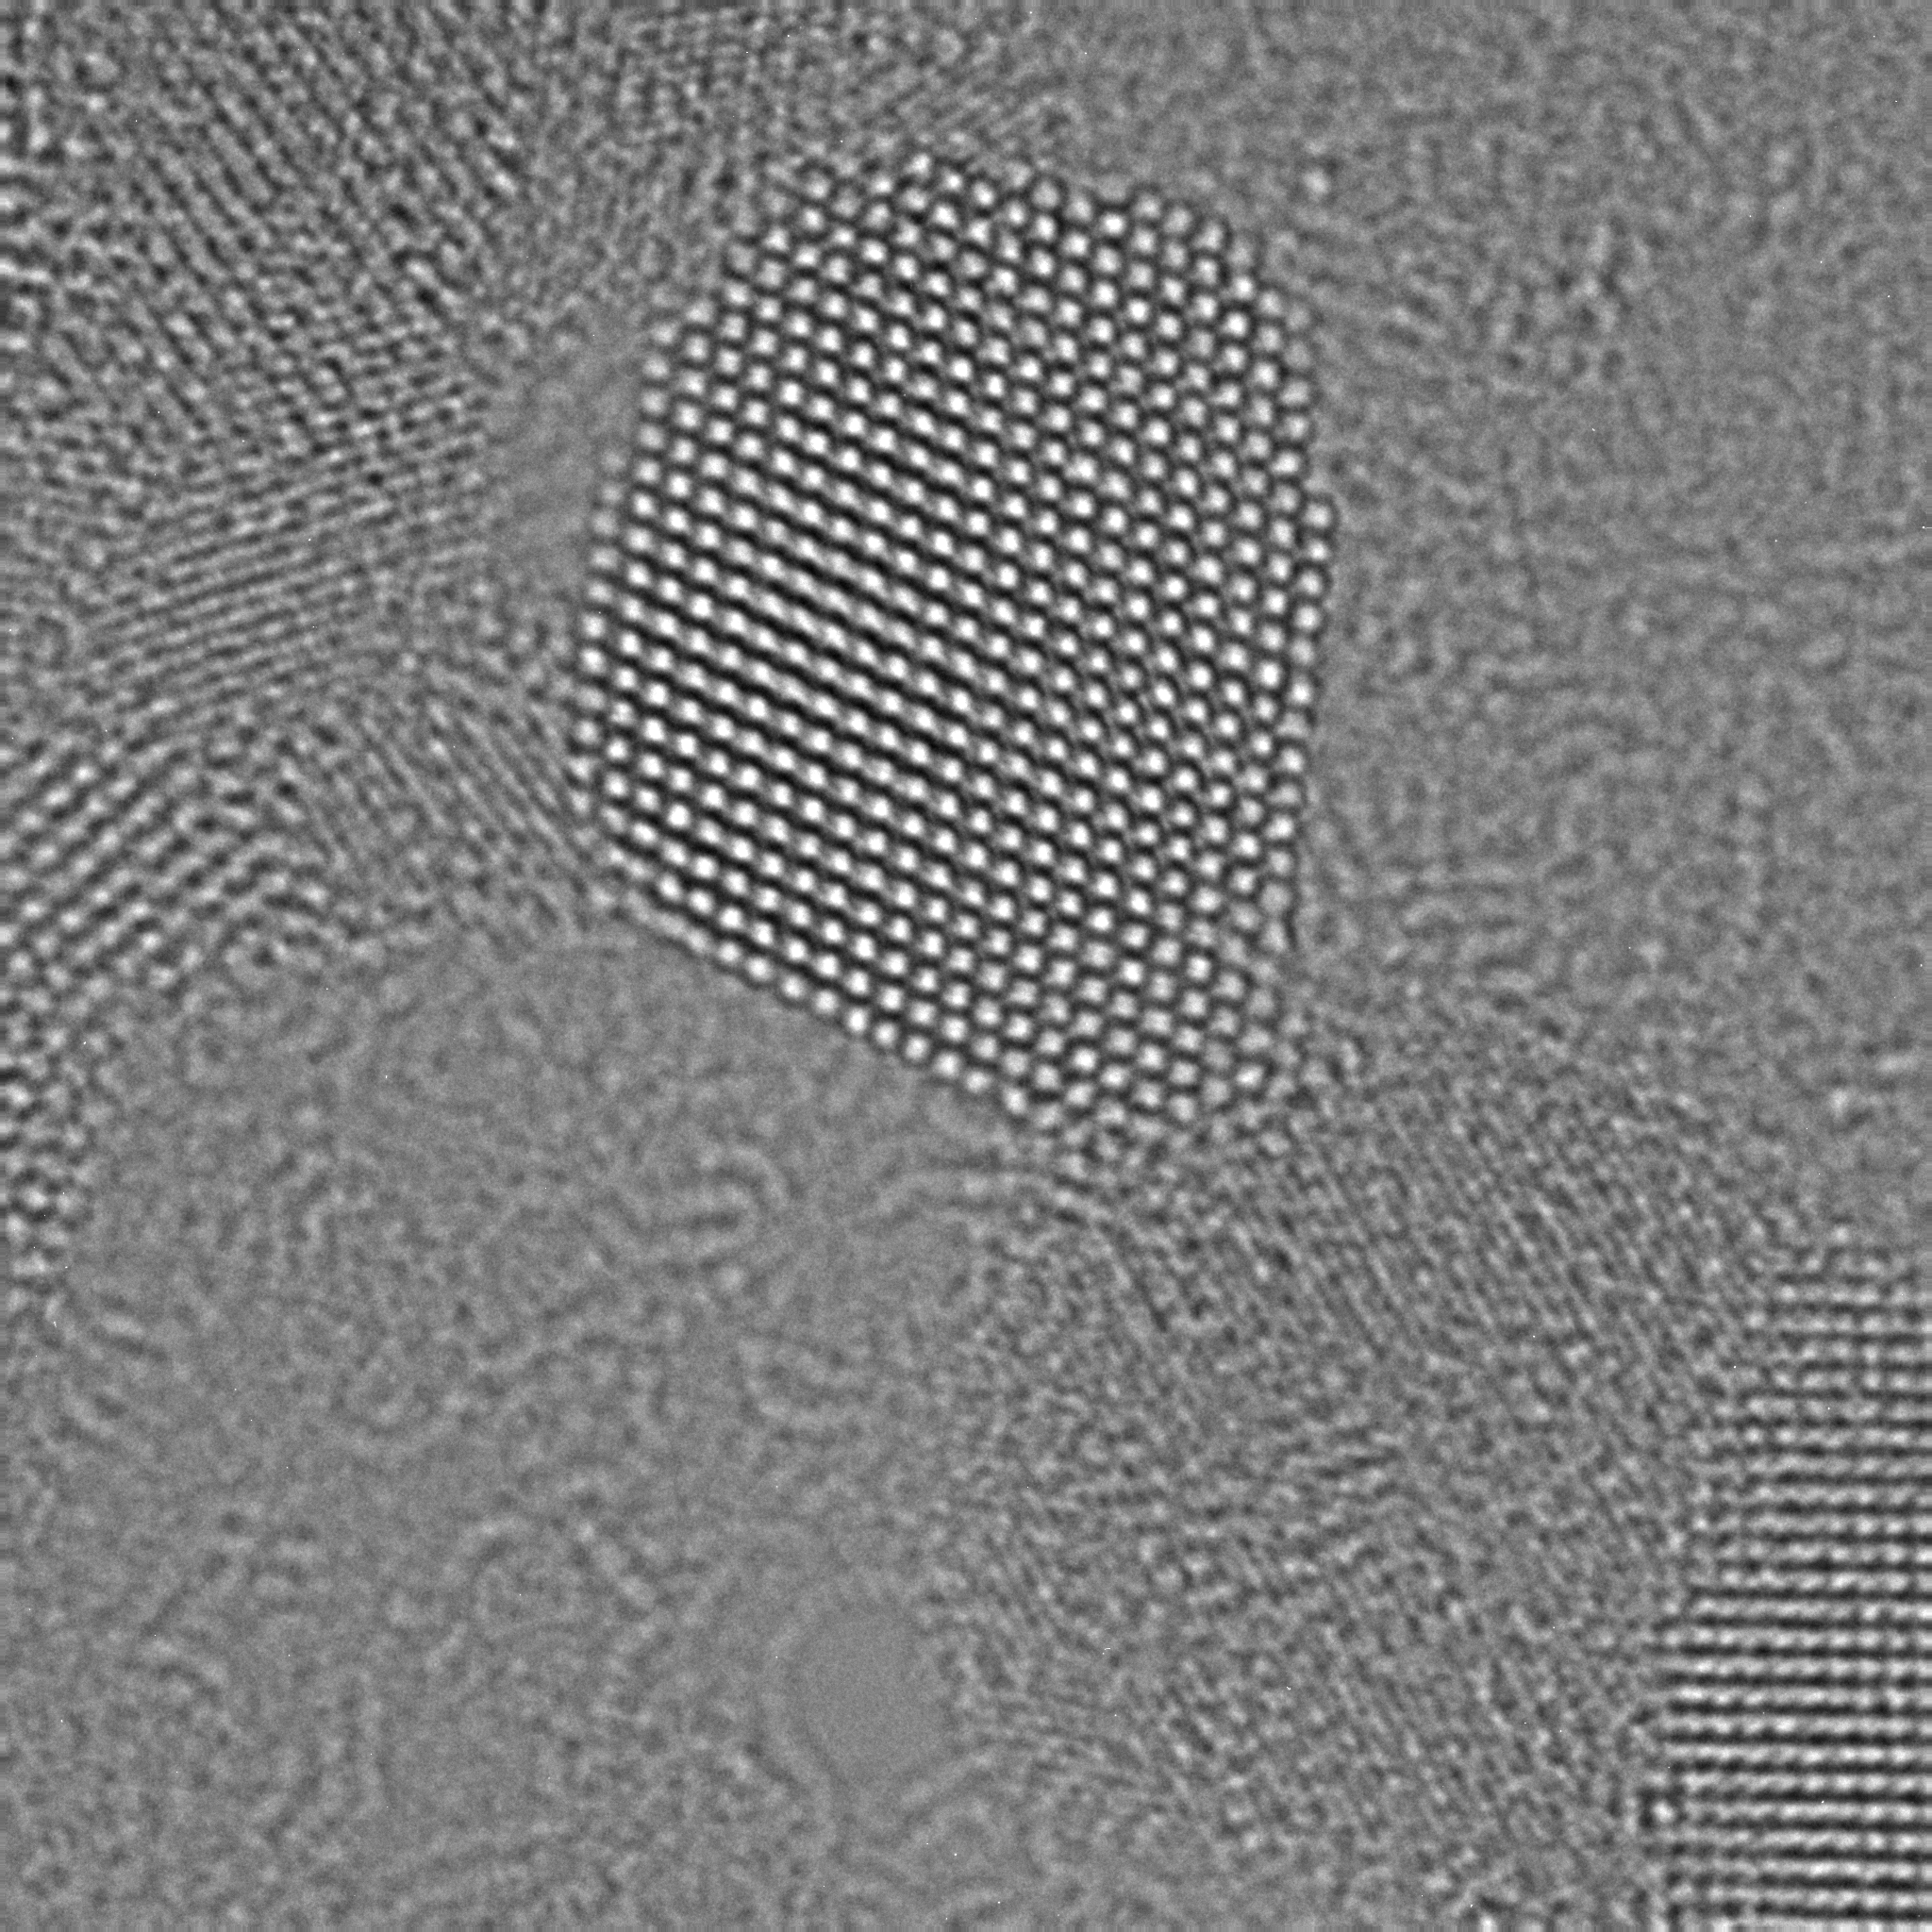
\includegraphics[width=0.5\textwidth]{img/T_CeO2_a.png}
			\caption[Im2Model sample 2D-TEM experimental image input]{Im2Model sample 2D-TEM experimental image input ( image of a CeO2 crystal ).}
	\label{fig:cerium_oxide_exp}
	\end{center}
	\end{figure}
	
	
	Im2Model heavily relies on image processing algorithms, which tend to be computationally heavy. Therefore, data access and data replication directly influence the algorithms efficiency.\par 
	
	Image management will be carried out by recurring to the OpenCV class \textbf{Mat}.  Mat has two data parts: (i) the matrix header, containing control information such as the size of the matrix, the method used for storing, the memory address in which the matrix is stored, etc, and a (ii) array containing the pixel values. 
	The matrix header size is constant. The array containing the pixel values varies in size from image to image.\par 
 The reference counting system of OpenCV, proves to be ideal for our specific image data transformations. For example, to create a region of interest (ROI) in an experimental image we just create a new header with the new boundaries, referring to only a subsection of the full experimental data, reducing the number of unnecessary copies of potentially large images.\par 
 Each Mat object has its own header, however the image data may be shared between two or more instances by having their matrix pointers point to the same memory address.
 
	
	Figure \ref{fig:cerium_oxide_exp} illustrates an example Im2Model 2D-TEM experimental image input.  
	
		
	
	\subsection{Image simulation}
	
	In order to assess the workflow listed in the chapter \ref{chapter:workflow}, a prototype implementation of the TEM image simulation recurring to Dr. Probe command-line software tools \citep{drprobe} was develop. A wrapper class was produced for each of Dr. Probe command-line tools:
	
	\begin{itemize}
	    \item Task 1 -- \textbf{celslc} -- responsible for the slices generation based on atomic structure data that can be supplied either in form of a CEL file or a CIF file. The orientation of the atomic structure, namely the  
	    zone axis and upward vector orientations and supercell size are also an input parameter.\par 
	    A preliminary crystallographic analysis by Im2Cr  \citep{asilva2016} of the experimental TEM image is necessary. In order to automate the slice generation process an configuration file manager was produced for the given tool.
	    \item Task 2 -- \textbf{msa} -- responsible for performing the multislice algorithm for a chosen input wave function and a given set of object transmission functions. The tool is controlled via a parameter list provided in a text file. In order to automate the electron wavefunctions calculation process an configuration file manager was produced for the given tool.
	    \item Task 3 -- \textbf{wavimg} -- responsible for  calculating image intensity distributions from electron wave functions for a given set of TEM imaging parameter. 
	    The tool is controlled via a parameter list provided in a text file, and requires a complex valued wave function as input data, produced by the prior multislice algorithm.
	    In order to automate the image intensity distributions calculation process an configuration file manager was produced for the given tool.
	\end{itemize}
	
	
	All the above command-line tools were pre-compiled for 64-bit Unix/OSX/Microsoft Windows operating systems for single-thread calculations, and therefore are not accountable for direct application performance improvements. The described command-line tools source code is currently inaccessible. \par 
	
	Given the described task chain for HRTEM image simulation, an example CeO2 ( cerium oxide ) nanostructure TEM simulated image was produced and it is presented on figure \ref{fig:sim_cerium_oxide}.
	
	%./im2model --cif=../simulation/cif/CeO2.cif --slc=test --prj_h=-2 --prj_k=-1 --prj_l=-1 --prp_u=-1 --prp_v=2.461462 --prp_w=-0.461462  --super_a=2 --super_b=2 --super_c=16 --nx=360 --ny=360 --nz=119 --ht=200 --dwf --abs  --slices_load=119 --slices_max=119 --defocus_samples=5 --defocus_lower_bound=-20 --defocus_upper_bound=20 --exp_image_path=../simulation/tif/T_CeO2_b_0.009nm.tif --exp_nx=0.009 --exp_ny=0.009 --roi_x=1072 --roi_y=937 --ignore_edge_pixels=30 --sim_grid --slices_upper_bound=100 --slices_lower_bound=10 --slices_samples=6 --roi_size=300 --cs=-17000 --cd=-8.5 --no_wavimg --no_celslc --no_msa
	
	\begin{figure}[!ht]
	\begin{center}
		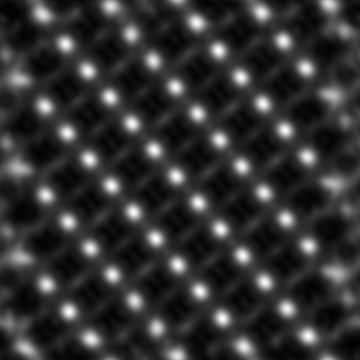
\includegraphics[width=0.5\textwidth]{img/003_002_Ce02_b_t__6dot18_d__-10.png}
			\caption[Example CeO2 nanostructure simulated image]{Example CeO2 ( cerium oxide ) nanostructure simulated image.\\
			Miller Indices  (hkl): [-2 -1 -1].\\
			Coordinates uvw: [-1 2.461462 -0.461462].\\
			Supercell size abc: 2 2 16.\\
			Ht: 200 kV.\\
			{$C_s$}: -17000.\\ 
			{$C_d$}: -8.5.\\
			Thickness: 6.18 nm.\\
			Defocus: -10 nm.
			}
	\label{fig:sim_cerium_oxide}
	\end{center}
	\end{figure}
	
	\subsection{Further simulated image transformations}
	
	
	The objective apertures, the spatial coherence of the beam and its wavevelenght have effect on border aberrations. Those aberrations may appear particularly remarked in the edges of the unit-cell, therefore compromising the achievable best correlation between the 2D-TEM experimental image and the simulated images.\par 
	A supercell model representing the hole nanostructure should only posses border aberrations on the outher shape and not on every unit cell. Those aberrations should therefore be eliminated by ignoring sufficient outter pixels from the simulated TEM images.\par 
	In order to proceed to the comparison with the experimental image, both experimental and simulated image must possess the same sampling rate. Each pixel must represent the same physical dimension expressed in nanometres per pixel (nm/px).\par 
	
	
	
		\begin{figure}[!ht]
	\begin{center}
		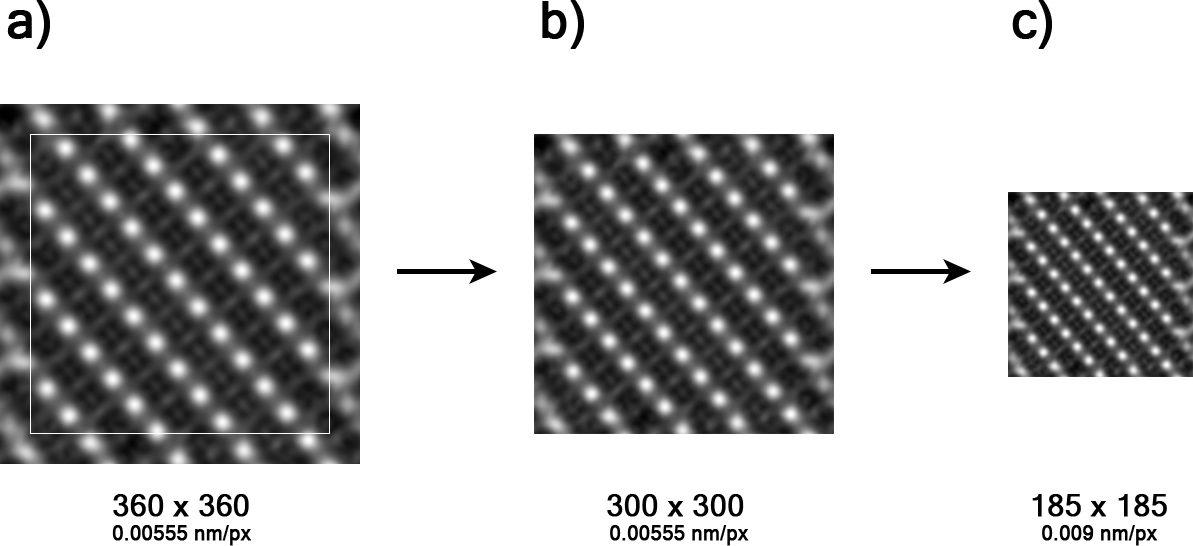
\includegraphics[width=0.75\textwidth]{img/sampling_rate_and_ignore_edges}
				\caption[Border aberrations of HRTEM simulated images]{Border aberrations of HRTEM simulated images.\newline 
				a) Simulated image of an CeO2 (cerium oxide) crystal.\\
			b) Cropped simulated image of an CeO2 (cerium oxide) crystal, given an crop size of 30 pixels.\\
			c) Final simulated image of an CeO2 (cerium oxide) crystal, following the crop and reshape operations.
			}
	\label{fig:sim_image_crop_factor}
	\end{center}
	\end{figure}
	
	
	
	Figure \ref{fig:sim_image_crop_factor} exemplifies the previously enumerated obstacles when there is a need to correlate simulated and experimental images. The simulated image posseses border aberrations, and both simulated and experimental images have different sampling rates (0.009 nm/px vs 0.0055 nm/px).\par 
	The initial simulated image, visible in figure \ref{fig:sim_image_crop_factor} a), will be cropped  by 30 pixels in every border directions. Given the sampling rate mismatch the already cropped simulated image, visible in figure \ref{fig:sim_image_crop_factor} b), will be reshaped  by a factor of 0.617284. The final simulated image, visible in figure \ref{fig:sim_image_crop_factor} c), presents a size of [185,185] pixels.
	
	
	

			
	
\subsection{T-focus map}
	

Both defocus and sample thickness have a significant effect on the image intensity distribution. In order to estimate the best fit to the experimental image of both parameters, several step-wise variations should be computed. Therefore, given an initial estimate of both the defocus and thickness variation ranges, and the desired sample number in order to discretize each continuous range interval, a 2D variation map is created. An example T-focus map of a CeO2 crystal is presented in figure \ref{fig:t_focus_map} b). 


\begin{figure}[!ht]
	\begin{center}

%./im2model --cif=../simulation/cif/CeO2.cif --slc=test --prj_h=-2 --prj_k=-1 --prj_l=-1 --prp_u=-1 --prp_v=2.461462 --prp_w=-0.461462  --super_a=2 --super_b=2 --super_c=16 --nx=360 --ny=360 --nz=119 --ht=300 --dwf --abs  --slices_load=119 --slices_max=119 --defocus_samples=5 --defocus_lower_bound=-20 --defocus_upper_bound=20 --exp_image_path=../simulation/tif/T_CeO2_b_0.009nm.tif --exp_nx=0.009 --exp_ny=0.009 --roi_x=1072 --roi_y=937 --ignore_edge_pixels=30 --sim_grid --slices_upper_bound=100 --slices_lower_bound=10 --slices_samples=6 --roi_size=300 --cs=-17000 --cd=-8.5


	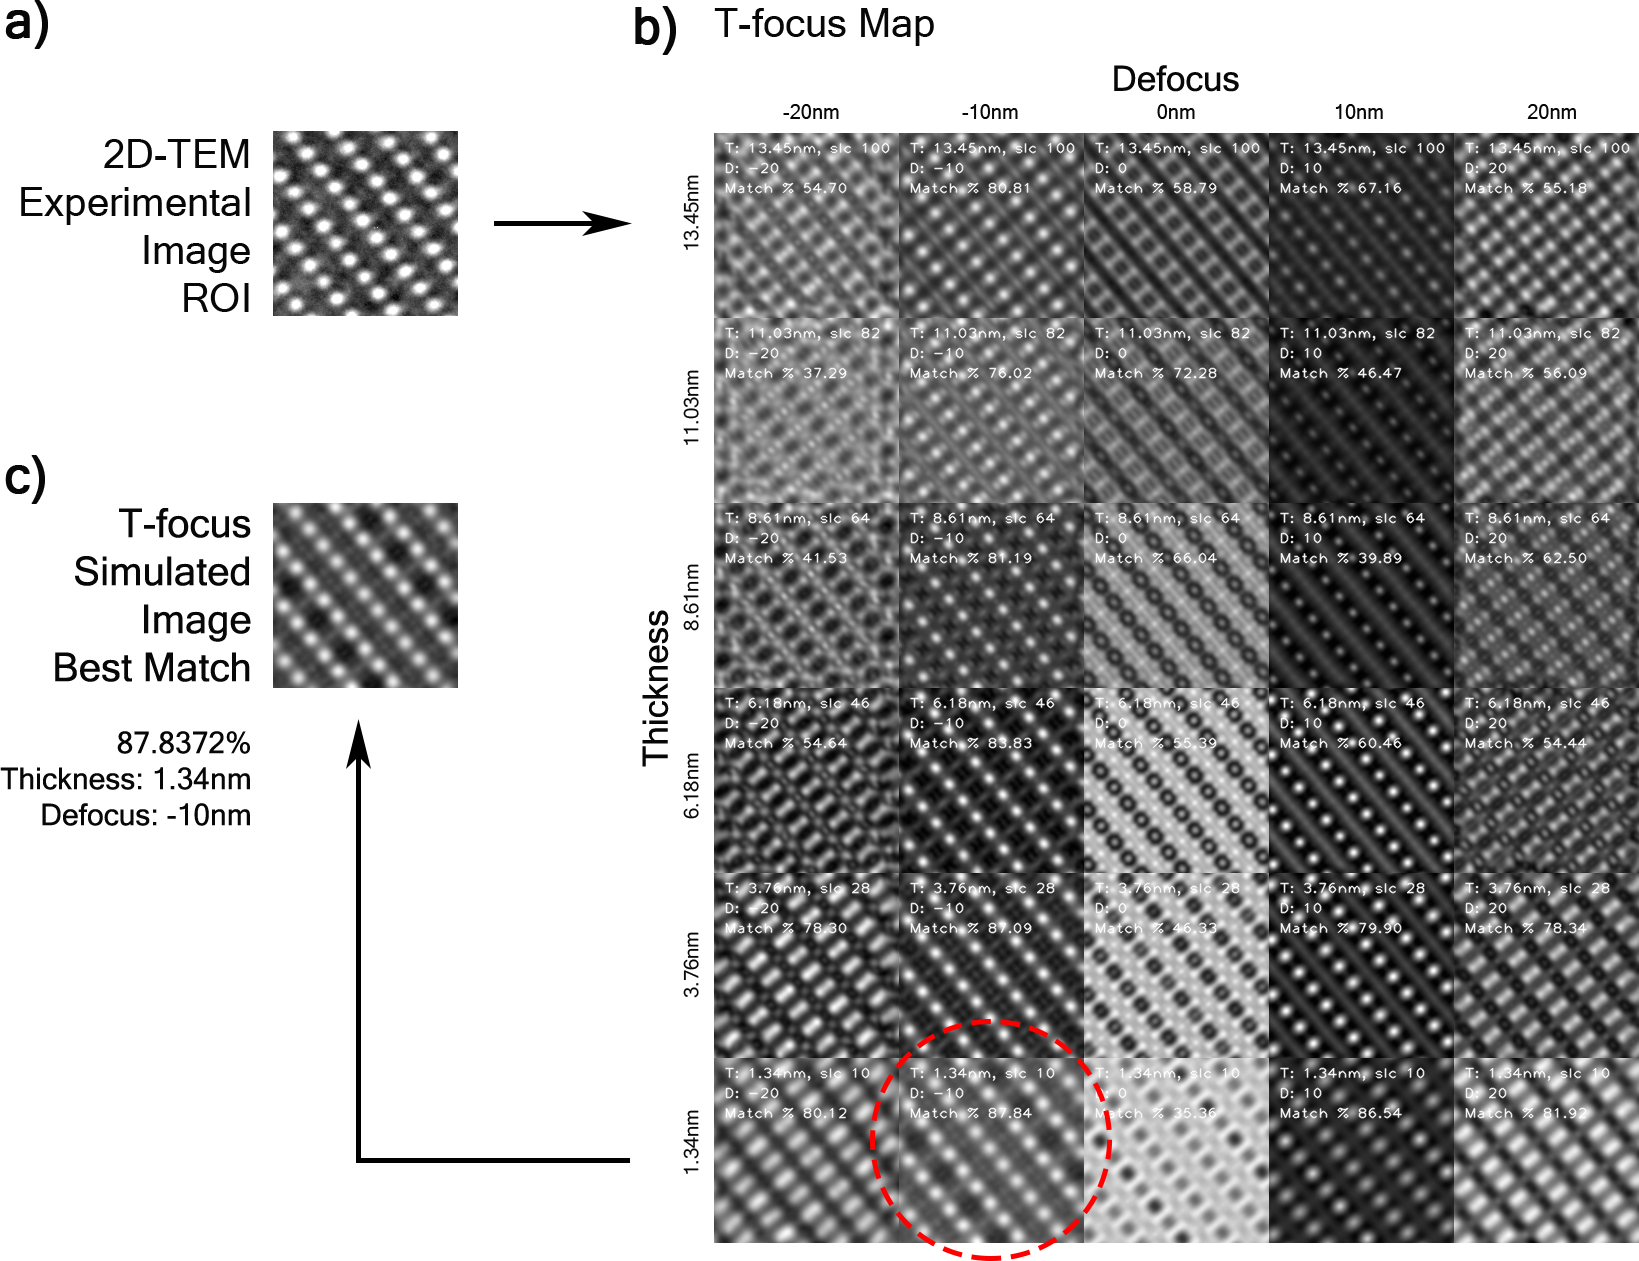
\includegraphics[width=1\textwidth]{img/t_focus_map.png}
			\caption[T-focus map of a CeO2 crystal]{T-focus map of a CeO2 crystal.\newline 
						a) Selected ROI from the 2D-TEM image.\\
			b) T-focus Map of a CeO2 (cerium oxide) crystal.\\
			Thickness variation interval (nm): [1.34,13.45], distinct thickness samples samples: 6.\\
			Defocus variation interval (nm) [-20,20], distinct thickness samples samples: 5.\\
			{Other experimental setup parameters: Miller Indices  (hkl): [-2 -1 -1], Coordinates uvw: [-1 2.461462 -0.461462], Supercell size abc 2 2 16, Ht 200 kV, {$C_s$}: -17000, {$C_d$}: -8.5.}\\
			{c) Thickness and Defocus best fit to the experimental image.}
			}
	\label{fig:t_focus_map}
		\end{center}
	\end{figure}

	Visual comparison between the give experimental image ROI and each of the simulated images present on the T-focus map can now be executed. To evaluate that comparison between the images we produced a 2-step correlation algorithm, with the first being a patch-based translation alignment recurring to a correlation coefficient, and the second step being an incremental refinement for the best given match in step 1, by enabling an euclidean translation transformation on that image.\par 
	Since Im2Cr \citep{asilva2016} crystallographic information may contain an certain amount of error regarding the angle differences between experimental and simulated images, the seconds step enables refined transformations in scale, angle and position. We can therefore confirm both Im2Cr \citep{asilva2016} inputs and user inputs regarding the sampling rate of the experimental image.
	\par 
	Figure \ref{fig:2d_planar_transformations} demonstrates the 2D planar transformations associated to the 2-step correlation algorithm. In the red dashed rectangle we can observe the search domain of the T0 patch image ( simulated image ) in I1 ( experimental image ). Step 1 is performer for all simulated images calculate in T-focus Map. \par 
	After the patch-based translation performed in step 1, we can now visualise the corresponding best match in the Experimental Image ROI (dashed yellow rectangle). Since minor errors may occur, due to either user input or Im2Cr \citep{asilva2016} input, the euclidean translation transformation enables further refinements in the correlation process.\par 
	Figure \ref{fig:2d_planar_transformations} b') and c') are the corresponding experimental and simulated images in which we should base the next steps of Im2Model.

	\begin{figure}[!ht]
	\begin{center}
		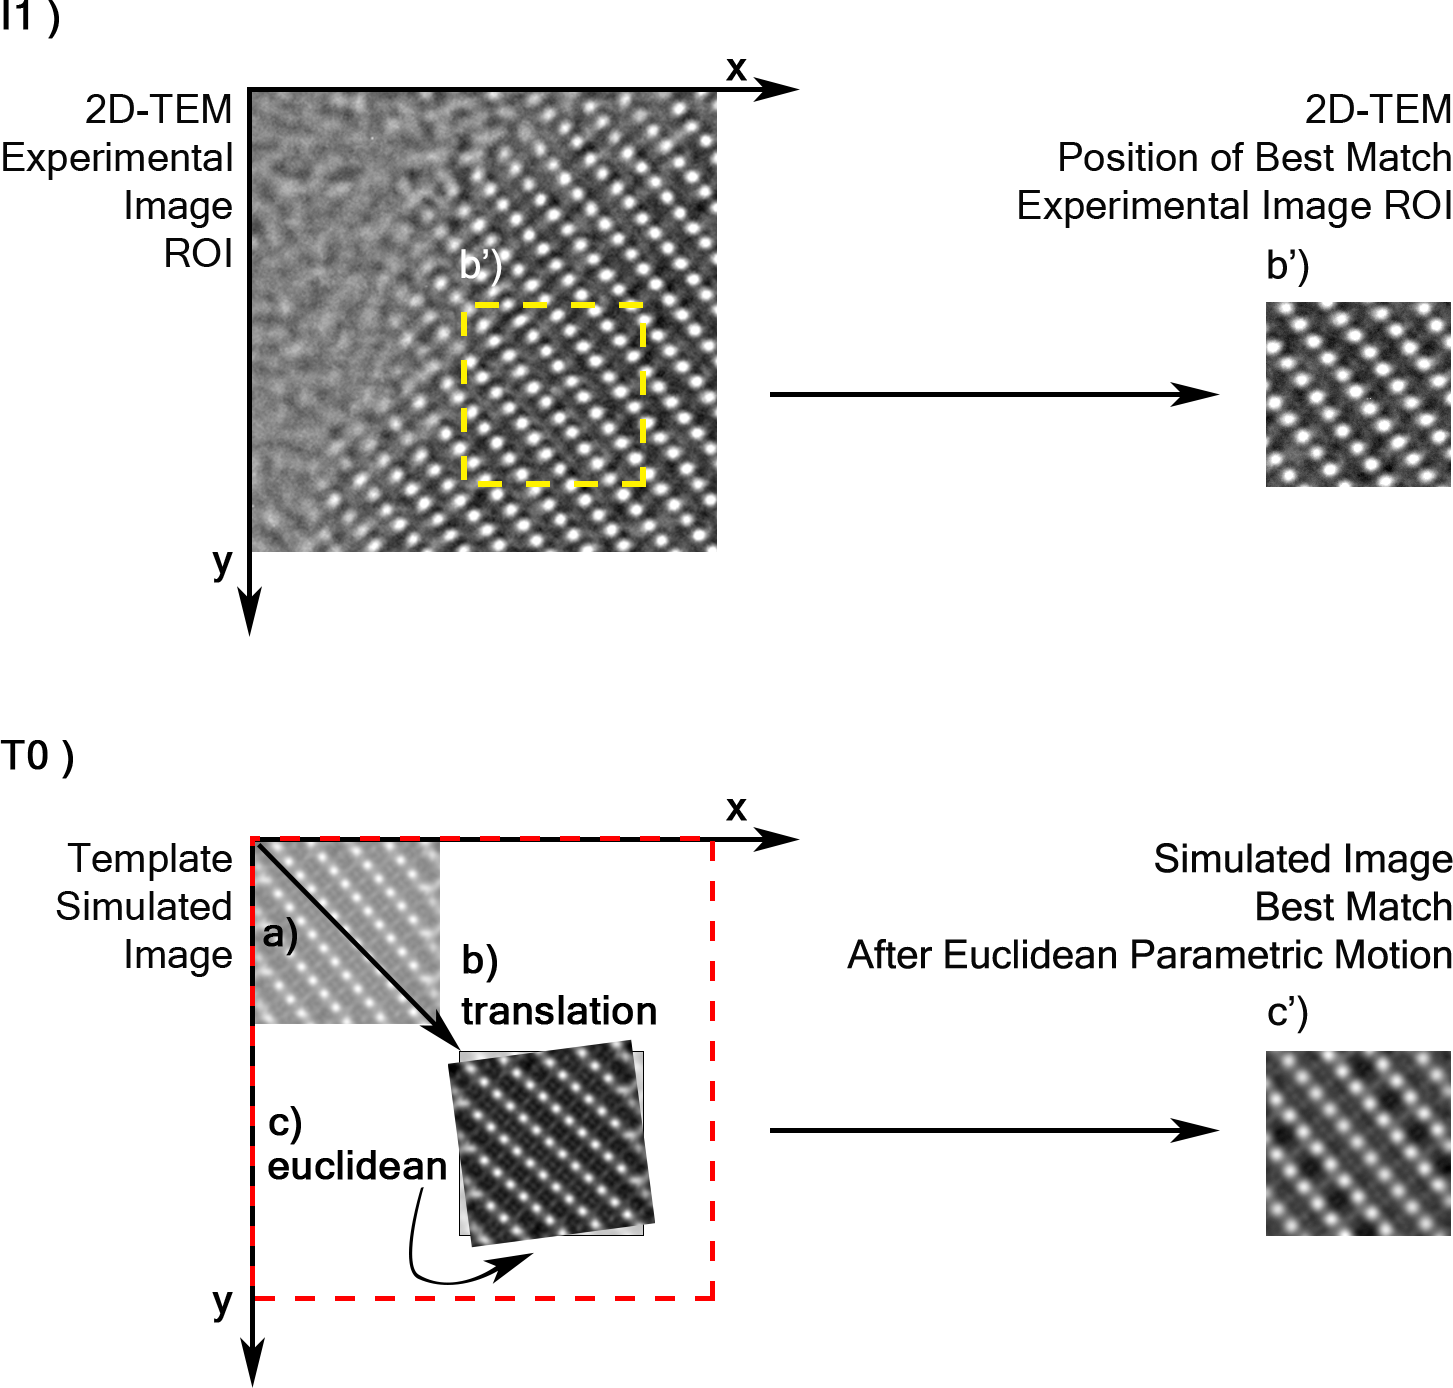
\includegraphics[width=0.9\textwidth]{img/2D_planar_transformations.png}
			\caption[2D planar transformations present on the 2-step image correlation algorithm]{2D planar transformations present on the 2-step image correlation algorithm.\\ 
			a) Template Simulated Image initial position.\\
			b) Template Simulated Image after patch-based translation alignment.\\
			b') Position of Best Match in the Experimental Image ROI.\\
			c) Template Simulated Image after euclidean translation transformation.\\
			c') Simulated Image Best Match after euclidean parametric motion.\\
			}
	\label{fig:2d_planar_transformations}
	\end{center}
	\end{figure}
	
	Given the best match calculated by the T-focus map, we can now have an estimation of the local thickness and defocus values for the given experimental ROI.\par 



	
\subsection{Supercell estimation}

\subsubsection{Outline of the X-Y crystal shape}


A typical way to compute edges in an image is to find local variations in intensity levels.
Recurring to the Canny edge detector algorithm \citep{canny1986computational}, a well known technique to find edges, we are capable of computing these derivatives and return an image with the approximated boundaries. \par
An area estimation of the X-Y crystal shape is also computed. Figure \ref{fig:edge_detection_exp} illustrates the Canny edge detector algorithm of an CeO2 ( cerium oxide ) crystal. 

\begin{figure}[!ht]
	\begin{center}
	
	\includegraphics[width=0.75\textwidth]{img/edge_detection_exp.png}
			\caption[Edge detection of the experimental image ROI algorithm visualization]{
			Edge detection of the experimental image ROI algorithm visualization.}
	\label{fig:edge_detection_exp}
		\end{center}
	\end{figure}
	
	% CHAPTER - Contribution -------------------------
		\section{Describing the problem}
		
	

Following the state of the art presented in chapter \ref{chapter:im2model_workflow}, this dissertation aims to apply the concepts presented and proven in the previous sections regarding the construction of atomic structures based on high resolution TEM images interpretation, and simulation of optical parameters correlating with the experimentally acquired image.



The Im2Model application should be structure trough the following steps:

\begin{itemize}
    \item \textbf{T-focus Map} -- Validation of the experimental setup parameters informed by the
user and the preliminary crystallographic analysis by Im2Cr \citep{asilva2016} of TEM images  through image simulations of a small segment and its
comparison with the experimental image, with the optical parameters varied stepwise in such a way that the image with the best fit to the experimental image will estimate the local sample thickness and defocus.\par This procedure is often referred as thickness-defocus maps in
TEM simulation, and 
will be carried out using Dr. Probe \citep{drprobe} %%pf verificar referencia
		command-line software tools, composed of three tools, each related to one of the three Dr. Probe simulation steps. Wrappers for the target operating systems will be created.\par  The best fit to the experimental image will be carried out by recurring to the free Open Source Computer Vision Library (OpenCV), with two step image correlation algorithms and their respective suitable error metric, the first being a patch-based translation alignment with the similarity metric being the normalized correlation coefficient, and the second being an more sophisticated euclidean parametric motion with the same similarity metric as the first correlation step.
		
		
\item  \textbf{Supercell estimation} --  A super cell model representing the whole structure will be built based on the crystallographic structure
retrieved by Im2Cr \citep{asilva2016} and the estimated dimensions of a certain region of interest. At a first step an outline of the X-Y crystal shape will be produced based on the ROI. A rough estimation of the 3D nanostructure will be achieved after this workflow step.\par 




\item \textbf{Supercell refinement} -- Iterative steps of image
simulation, images comparison and model refinement will be carried out until a convergence threshold. Input parameters will also be refined and validated.\par  
\end{itemize}



During these steps, the atomic model and the TEM experimental parameters will be refined, leading to a
complete description of the sample structure. We should have an atom by atom description of the nanostructure.\par 	

		\section{Component architecture}

			\subsection{Dependency analysis}


%In this method if a pixel has a value above the high threshold them it belongs to an edge, if the value is bellow the low threshold it does not belong to an edge and if it is in between it belongs to an edge if it is connected to a pixel with value above the high threshold.:



\chapter{Efficient implementation of Im2Model workflow}
		    \section{Describing the final goal}
		    Im2Model main objective is to provide a time-efficient and
unbiased work-flow for the quantitative interpretation of high-resolution TEM images, by the use of
efficient computation methods, enhancing the productivity on materials characterisation at the atomic
scale.
The resource utilisation efficiency for a given application workload
can be considered as the secondary objective.\par 
	
	In order assess Im2Model efficiency on the prior metris  a theoretical performance model should be developed. Based on it we could impose theoretical performance roofs, explain experimental results and provide direction for the next software improvement step.
	
		    \subsection{Modelling the bootlecks}

		    \section{Modelling the solution}
		    \subsection{Designing the data model}
		    \subsubsection{Storage and retrieval}
		    \subsubsection{Distributed data}
		    		    \subsection{Designing the application model}

		      \subsubsection{Designing for testability}
		      
		      
		    \section{The trouble with the modelled solution}
		    \subsubsection{Unreliability}
		    \subsubsection{Distributed data}
		    
		    

\chapter{The test boundary}

	% CHAPTER - Conclusion/Future Work --------------
	\chapter{Conclusion}


Im2Model has for main objective to provide a time-efficient and unbiased worflow for the quantitative interpretation of HRTEM images. The major challenge regarding this pre-dissertation work frame was perceiving the essential nanomaterials theory in order to fully understand the challenges and efforts towards the main goal completion. This process was longstanding and it was only managed
to do it with help of both advisors.\par 


Concerning the performance modelling, several potential exploratory
paths can be taken, leaving the essential performance-related decisions to post Im2Model software requirements completion.\par 

The Im2Model workflow has been fully characterised, and it is now time to complete the remaining steps and to "think towards efficiency and parallel".


		    \section{The future of im2model}
		    
		     \subsection{Integrations}
		     
		      \subsection{Aiming for observality}
		      
		      \subsection{Trusting, but verifying}
		      
		      \subsection{Privacy, Tracking, and Compliance}

	\bookmarksetup{startatroot} % Ends last part.
	\addtocontents{toc}{\bigskip} % Making the table of contents look good.
	%\cleardoublepage

	%- Bibliography (needs bibtex) -%
	\bibliography{dissertation}

	% Index of terms (needs  makeindex) -------------
	%\printindex
	
	
	% APPENDIX --------------------------------------
	\umappendix{Appendix}
	
	% Add appendix chapters
%	\chapter{Support material}
%	Auxiliary results which are not main-stream; or

	%\chapter{Details of results}
%	Details of results whose length would compromise readability of main text; or

	%\chapter{Listings}
%	Specifications and Code Listings: should this be the case; or

	%\chapter{Tooling}
%	Tooling: Should this be the case.

	%Anyone using \Latex\ should consider having a look at \TUG,
	%the \tug{\TeX\ Users Group}


	% Back Cover -------------------------------------------
	\umbackcover{
	%NB: place here information about funding, FCT project, etc in which the work is framed. Leave empty otherwise.
	}


\end{document}
